\chapter{Suitability Benchmark}\label{experiment}

It is not enough to look at produced explanations and draw conclusions.
We must carefully establish evaluation criteria to verify that the reviewed methods are faithful and comprehensible proxies of our model.
First, we outline what a good explanation should fulfill.
Then, we address the current problem of high computational resource utilization of Occlusion.
In the third section, we construct a quantitative benchmark, choosing appropriate metrics alongside a brief rationale and evidence for our choice.
In the last section, we perform a subjective evaluation by a domain expert.

We will use implementations from XAI-oriented machine learning libraries, \texttt{captum}\footnote{\url{https://github.com/pytorch/captum}} (Occlusion, Composite-LRP), \texttt{torch-cam}\footnote{\url{https://github.com/frgfm/torch-cam/}} (CAM), and \texttt{pytorch-grad-cam}\footnote{\url{https://github.com/jacobgil/pytorch-grad-cam}} (HiResCAM, GradCAM++, ScoreCAM, AblationCAM).
For the implementation of the benchmark into the \texttt{prostate-cancer}\footnote{\url{https://gitlab.ics.muni.cz/rationai/digital-pathology/pathology/prostate-cancer}} pipeline, see \myref{Section}{sec:imple}.

CAM-based methods can compute saliency maps for our model's arbitrary convolutional or pooling layers.
Given the notion of a hierarchical representation with increasing complexity towards deeper layers, attributing the lower layers does not make sense when trying to find concepts recognized by a domain expert.
Instead, we examine the final convolutional and pooling layers.
We used the pooling layer based on the results of an additional experiment in \myref{Section}{sec:conv-vs-pool}.

For Composite-LRP, the configurations are countless. We based our setup on \myref{Figure}{fig:lrp-montavon}, but decided to replace the LRP-$\gamma$ rule for LRP-$\alpha\beta$ rule from \cite{lrp-alpha-beta}, which produced visually sharper results.
Despite our efforts, the resulting saliency maps are still notably scattered, and we decided not to spend too much time exploring different options since we believe the method will not outperform Occlusion.

\pagebreak

\section{What makes a good explanation?}

\begin{quote}
    \emph{``Unfortunately, `explainability' is a nebulous and elusive concept that is hard to target.''} \cite{explainability-hard}
\end{quote}

Contemporary research does not provide a unified approach to measuring the ``goodness'' of an explanation.
There are attempts to propose a set of properties that a good explainability method should fulfill, but they are not aligned \cite{xai-functionality-grounded, explainability-hard, xai-meta-survey, xai-zhou-survey}.
According to Doshi-Velez and Kim in \cite{xai-doshi}, ``the field is crowded with evaluation methods, and there is no consensus on which are the `right' ones. 
Much less, there is not even agreement on which criteria should be evaluated''.
The challenge lies in the absence of ground truth for produced explanations, and therefore, we have no objective measure of grading the explanations \cite{xai-zhou-survey}.
However, according to \cite{xai-anecdotal-evidence}, we can avoid so-called ``anecdotal evidence'' and argue that specific explainability methods are sufficient given the audience and the use-case by carefully choosing the metrics by which we evaluate them.
We believe that for an explanation to be suitable to our use-case of generating slide-level explanations, it needs to be:
\begin{enumerate}
    \item Performant: This is the main bottleneck of the current solution. We do not care how good a method is without reasonable performance since we cannot utilize it for practical purposes to assist a pathologist and not disrupt his workflow.
    \item Faithful: Ideally, we want to ensure that the explainability method only highlights the regions of the input tiles that the model deems important for its decision.
    \item Useful: We need the explanations to be presented to domain experts so that it is understandable for them. If they do not understand the explanation, it is of little value. 
\end{enumerate}

\section{Computational Performance}

For an explainability method to actively assist a pathologist, the explanations must be computed fast enough.
The main limitation of the existing approach using Occlusion is to generate explanations for an entire slide in a reasonable time.
The problem is two-fold; we perform one forward pass with the occluded tile at a time, needing $289$ synchronous forward passes, or batch several occluded tiles together, drastically raising graphics processing unit (GPU) memory costs.
But even with internal batching, Occlusion is too slow to be used in real-time.
To tackle this problem from both perspectives --- we first measure the time it takes a method to produce a single explanation and then observe how much GPU memory the method uses.

\subsection*{Time Efficiency}

 We let each method fully explain the average size WSI of $1,499$ tiles from the test set.
 Although we aim for good slide-level performance, we measure the time required for individual tile-level explanations instead.
 During the generation of slide-level explanations, there are many auxiliary operations to combine tile-level saliency maps.
 Methods and their implementations are not responsible for these operations.
 We include this overhead if we measure the time required to generate slide-level saliency maps.
 Since modern machine learning frameworks typically use parallel processing employing multiple CPU cores, this can lead to resource locks, which can negatively affect the performance of a method if we consider the required slide-level time.
 Another reason for measuring the time required for tile-level explanations is resource saving.
 We want to take multiple unit measurements and see their mean and variance, as momentary factors of the machine environment can influence a single data point. 
 By taking multiple data points, we hedge against these factors.
 If we were to measure the slide-level performance, it would be much more time-consuming, blocking resources from other students and colleagues in the RationAI group.

 We performed a run for each method on a machine with $8$ cores, $16$GB of RAM, and a single NVIDIA A40 GPU card with $48$GB of memory.
 For Occlusion, we used the internal batch size of $200$ perturbed tiles.
 Other methods do not offer this option.
 We repeatedly fed each method a single tile and measured the time difference between the start and end of the saliency map computation.
 After the method call, we inserted a \texttt{torch.cuda.synchronize} call to ensure that computation on GPU was complete before taking the end-of-computation timestamp.

\begin{table}
\centering
\ra{1.2}
\begin{tabular}{@{} l @{\ }r r r @{}}\toprule
Method & Avg. time per tile (s) & Time for slide & Expected largest slide time \\ 
\midrule
CAM                 & $0.04 \pm 0.04$ & $0.99$ m   & $2.73$ m \\
GradCAM++           & $0.08 \pm 0.00$ & $2.19$ m   & $6.05$ m \\
HiResCAM            & $0.08 \pm 0.00$ & $2.20$ m   & $6.06$ m \\
Composite-LRP       & $0.11 \pm 0.00$ & $2.98$ m   & $8.21$ m \\
\textbf{Occlusion}  & $1.06 \pm 0.00$ & $26.87$ m  & $1.23$ h \\
AblationCAM         & $9.72 \pm 0.00$ & $4.05$ h   & $11.16$ h \\
ScoreCAM            & $9.76 \pm 0.00$ & $4.06$ h   & $11.19$ h \\
\bottomrule
\end{tabular}
\caption{
The time efficiency of the XAI methods reviewed in \myref{Section}{sec:xai-cnn}.
We have ordered methods from the fastest to the slowest.
The entry for Occlusion is in bold to visually separate the methods into faster and slower than the current solution.
Unsurprisingly, methods that require a single pass to compute the importance of activation maps were the fastest, while the methods that perturb either input or model internals were slower, as they require multiple forward passes to estimate the importance.
We could solve this, as in the case of Occlusion, by batching multiple perturbed inputs together, but the libraries do not provide such an option.
Even then, we would run into another problem; such batching requires tremendous GPU capacity.
The third column represents the estimated time to explain the largest slide from the test split to give an approximation of the current worst-case scenario of $4131$ tiles per slide.
}
\label{tab:comp-time}
\end{table}

\myref{Table}{tab:comp-time} shows the superiority of CAM methods that require a single forward pass to compute the saliency maps.
As expected, ScoreCAM performed the worst.
The time taken is due to the fact that for each of the $512$ activation maps of the last layer of our model, ScoreCAM performs a separate forward pass with a perturbed input tile.
The problem of multiple forward passes is tamed by batching in the case of Occlusion, where most of the overhead comes from creating perturbed tiles.
What surprised us was the time AblationCAM took to compute a single explanation.
\myref{Equation}{eq:ablation-cam-importance-weight} shows that the importance weights in the case of AblationCAM are computed by perturbing models internals --- systematically setting activations across layer units to zero.
In the case of our model, computing the importance weight for unit $k$ means setting the pooled activation $a^k$ to zero --- the output $y^c_k$ is simply a linear combination of pooled activations, omitting the $a^k$, which we would expect the library to compute reasonably quickly.

Since both AblationCAM and ScoreCAM performed significantly worse than Occlusion and did not bring us closer to finding a high-performance XAI method, we decided not to include them in further benchmarks.

\subsection*{GPU Utilization}

Modern GPUs offer the ability to run multiple processes simultaneously on the same card instance.
The demand a method places on GPU memory is critical to production deployment.
High GPU utilization by one method can limit the number of processes that can run in parallel, which, in turn, may increase deployment costs due to the need for additional GPU cards.
As neural networks are generally expensive to run in terms of energy consumption, their use leads to questions regarding their sustainability.
We should consider sustainability, a key concern in technology development and deployment today, when considering our models' future use and development.
We are unaware of previous work focusing on GPU utilization of explainability methods.
Still, given EU regulations from \myref{Section}{sec:need-for-xai}, we posit that we should evaluate it accordingly.
Failure to take these requirements into account could have a negative impact on the deployed models, as being unable to facilitate given restrictions may require them to be brought down.

As with the time efficiency metric, we let each method explain a single WSI of $1,499$ tiles.
We monitor the GPU usage by running the \texttt{nvidia-smi} executable in a separate process, forwarding its output to a CSV file every $500$ milliseconds.
\myref{Table}{tab:gpu-util} shows the utilization of a single A40 GPU card while the explanations are being computed.
Note that we cannot distinguish exactly which part of the GPU memory the XAI method uses, as we also store the model on the GPU.
For this reason, we performed one run without computing any explanations to serve as a baseline.
We ran all of the runs with a batch size of one to avoid discriminating between methods.
We expect all methods to score better than Occlusion, as none rely on internal batching.

The results in \myref{Table}{tab:gpu-util} confirm our expectations that none of the methods except Occlusion noticeably exhaust the GPU.
Therefore, we can run multiple processes simultaneously on a single card instance using one of our candidate methods.
Furthermore, the smallest GPU RationAI has at its disposal, with a capacity of $10$GB, is enough to facilitate all candidate methods, which is not the case for Occlusion.
\begin{table}
\centering
\ra{1.2}
\begin{tabular}{@{} l r r @{}}\toprule
Method & Absolute GPU utilization (MB) & Relative Overhead (MB) \\ 
\midrule
Baseline run       & $910$      & -       \\
CAM                & $1084$     & $174$   \\
GradCAM++          & $1,578$     & $668$   \\
HiResCAM           & $1,578$     & $668$   \\
Composite-LRP      & $2,476$     & $1,566$  \\
\textbf{Occlusion} & $36,308$    & $35,398$ \\
\bottomrule
\end{tabular}
\caption{
GPU utilization of the reviewed XAI methods.
We use mode instead of mean because, after two GPU memory usage snapshots, the number remains the same until the end of the benchmark.
The Absolute GPU utilization column captures the raw output of the \texttt{nvidia-smi} command, while the Relative Overhead column corresponds to the additional consumed memory on top of the standard model's requirements.
All values are in megabytes.
All methods performed better than Occlusion, which we attribute mainly to not running batched forward passes.
CAM achieved the lowest utilization since it only multiplies activation maps with FC layer weights.
GradCAM++ and HiResCAM need to compute and retain specific gradients, which require more memory than vanilla pass.
Composite-LRP runs a complete backward pass equivalent and needs to hold the forward pass activations to compute relevance scores.
}
\label{tab:gpu-util}
\end{table}


\section{Quantitative Evaluation}\label{sec:quant}

This section discusses and evaluates two well-established metrics that capture the desired properties of explainability methods.
We build on the work of Gallo et al. \cite{gallo} by incorporating state-of-the-art metrics that address the limitations of previous approaches.
By refining previously used metrics, we aim to provide a more reliable benchmark while aligning the quantitative assessment with domain-specific boundaries.

\subsection*{Faithfulness}

A common approach to assess whether an explainability method is pointing to the relevant regions of the input image is to perturb the image by removing features that the method considers important and filling the removed areas with a fixed value  --- similar to how Occlusion estimates feature importance --- and observe how the model's confidence changes.
However, \cite{roar} suggests that this perturbation approach, which involves filling the removed areas with zeros or the mean pixel value, could be flawed.
The perturbed input could contain artifacts that compromise the reliability of such metrics since we cannot tell how much of the change in the model's confidence stems from introduced artifacts compared to the original relevance of removed features.

The experiment in \cite{gallo} utilizes methods prone to introducing such unintentional artifacts (Causal Deletion \cite{xai-causal-deletion} and Area Over Perturbation Curve \cite{xai-aopc}).
In particular, Occlusion and Deep-Taylor Decomposition \cite{xai-dtd} received the highest scores.
This result is aligned with the observation by Hsieh et al. \cite{xai-hsieh-occ-dtd} --- that such metrics may favor methods that rely on the exact mechanism when estimating the importance of input features.
As Occlusion estimates input feature importance by observing the decrease in the model's confidence on a perturbed image --- when we later remove a highly salient region, the model's score will inevitably drop.

Hooker et al. \cite{roar} introduced an alternative metric known as Remove and Retrain (ROAR), which involves zeroing out the identified important features and then retraining the tested model with the modified dataset --- observing the new performance.
Although ROAR has gained in popularity, it has the disadvantage of being computationally expensive, rendering it unacceptable for our use case.
As further shown by Rong et al. \cite{road}, ROAR does not solve the problem of the so-called \emph{class information leakage} --- the phenomenon when the uniformly-valued removed region reveals relevant class information through its shape.
Rong et al. \cite{road} propose a method that builds on the foundations of ROAR, called Remove and Debias (ROAD).
Instead of retraining the model, regions after removed features are specifically imputed to reduce the risk of class information leakage.
Refer to \cite{road} for mathematical intrications of information theory behind the imputation.

To evaluate the performance of our methods, ROAD iteratively removes features from the most relevant to the least (MoRF order) for specified percentages.
After each removal, missing features are imputed using a noisy linear imputer to reduce class information leakage \cite{road}.
For a single tile $x$, saliency map $S$ and percentage $p$, the result of this method is a number $d$ corresponding to the drop in confidence of a model computing function $f$ on the imputed tile
\begin{equation}
    d = f(x) - f\bigl(\operatorname{perturb}_p(x, S)\bigr).
\end{equation}
The function $\operatorname{perturb}_p$ takes the input image $x$, saliency map $S$, and imputes the regions corresponding to the top $p$ percent of most salient pixels of explanation $S$.

As in one of the experiments in the original paper, we evaluate our methods at $10, 20, 30, 40$, and $50$ percent of the most salient perturbed pixels.
While some other experiments in \cite{road} use imputation up to $85$ percent, this is not computationally feasible in our setting.
Computing the scores for our $5$ percentages already takes up to $4.5$ days for a single method.
Since our methods tend to cover larger areas of input tiles, imputing $85$ of the most salient pixels for a single tile takes about $11$ seconds, adding more than $3$ days to the computation time for a single method.
Furthermore, removing such a large portion of the tile leaves us with very few original features, and we are not sure how to interpret the drop in confidence in such a setting.
Considering those factors, we decided not to extend the perturbation beyond the $50$ percent of the most salient pixels.

According to \cite{road}, when evaluating a method, we want the model's score to drop significantly as we start to remove the features based on the generated saliency map and the rate to slow down as we approach the higher percentages, signaling that the key areas were indeed imputed in the beginning.
We evaluated our model using the \texttt{pytorch-grad-cam} package that provides the \texttt{NoisyLinearImputer} class.
This class is designed to handle the imputation of missing values in the same manner as the original implementation from the ROAD paper.
We did not use the original implementation\footnote{\url{https://github.com/tleemann/road_evaluation/tree/main/road}} from \cite{road} because the interface did not fit into our data-processing pipeline.
\myref{Figure}{fig:road-impute} shows how the \texttt{NoisyLinearImputer} imputes removed areas.
As this method relies on sensitivity, we only used the $24,858$ positive tiles from the test split of the dataset from \myref{Section}{sec:dataset}.
To see the curve of the drop in the model's confidence, refer to \myref{Figure}{fig:road-curve}.
We present a boxplot showing the distribution of our results in \myref{Figure}{fig:road-boxplot}.

Our results are consistent with the results of faithfulness metrics in \cite{gallo} --- ROAD tends to prefer techniques that identify broader, continuous regions within the input tile.
According to \myref{Figure}{fig:road-boxplot}, CAM-based methods produce more consistent results than Occlusion-based saliency.
Similar to $\varepsilon$-LRP in \cite{gallo}, Composite-LRP performs worse than Occlusion, rendering our efforts to assign different relevance rules to produce more coherent saliency maps according to \cite{lrp, lrp-alpha-beta} unsuccessful.
As shown in \myref{Figure}{fig:road-impute}, the tile imputed based on the explanation generated by Occlusion looks visually more distressed than the tile imputed according to the more scattered Composite-LRP method.
An interesting observation is that perturbation based on saliency maps produced by Occlusion and CAM does not increase the model's confidence, which is not the case for the other methods.
We also posit that despite the authors of GradCAM++ and HiResCAM promoting their methods as more faithful than CAM/GradCAM, it seems not to be the case, given our model and domain.

\begin{figure}
    \centering
      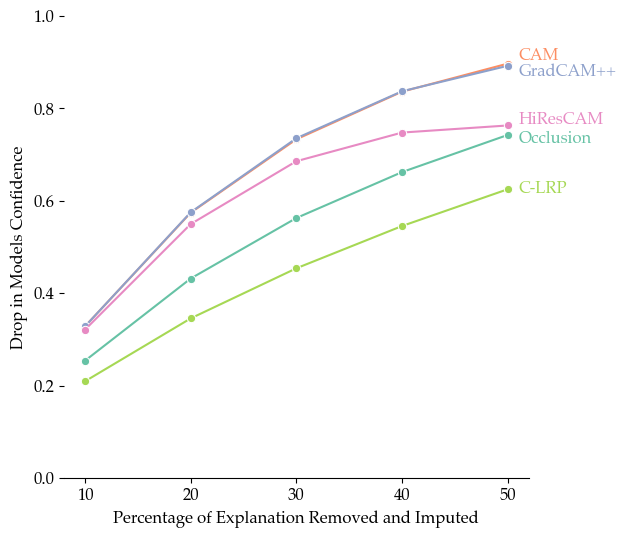
\includegraphics[width=0.7\textwidth]{img/road-curve.png}
    \caption{
    The curves visualize each method's mean drop in confidence per imputed percentage of most salient pixels.
    Note that CAM and GradCAM++ appear to be methods with similar performance when looking only at the mean.
    HiResCAM shows the desired behavior: the curve flattens as we impute larger fractions on the input.
    However, it achieves lower scores than other CAM-based methods.
    Composite-LRP underperforms Occlusion, per our prior expectations and results from \cite{gallo}.
    }
    \label{fig:road-curve}
\end{figure}

\begin{figure}
    \centering
      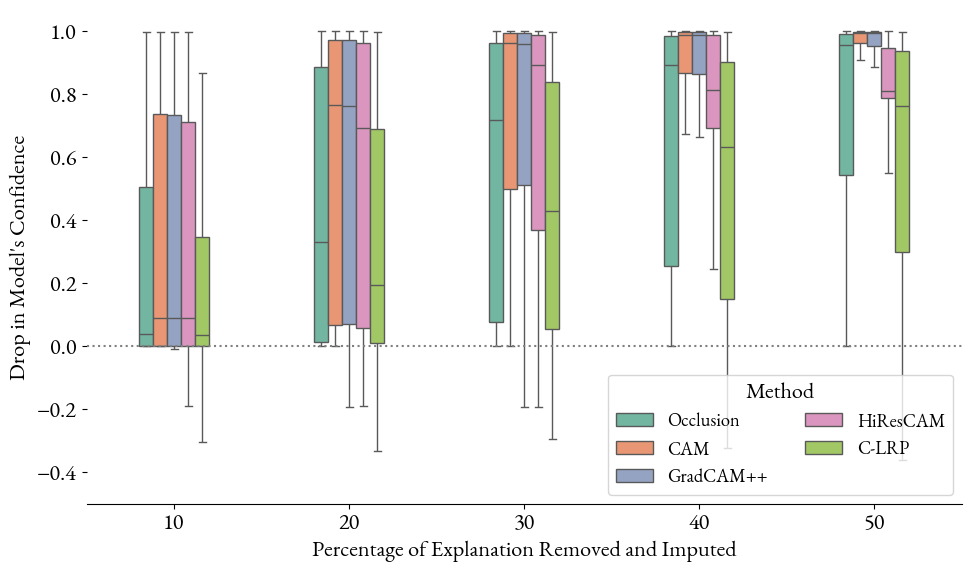
\includegraphics[width=\textwidth]{img/road-boxplot.png}
    \caption{
    Boxplot of results for our percentages of the ROAD method.
    We used the percentages from one of the experiments in \cite{road}.
    ROAD ranks CAM-based methods over Occlusion and Composite-LRP.
    We can see that perturbation by CAM-based method explanations decreases the model's confidence faster than the Occlusion method --- advocating for those explanations to be more faithful as they better localize important features.
    Scores for CAM methods also have less spread when significant parts of salient areas are removed.
    Notice the minimum values and that only CAM and Occlusion do not increase the model's confidence upon evaluation of perturbed tile, while gradient-based CAMs and Composite-LRP do.
    }
    \label{fig:road-boxplot}
\end{figure}

\begin{figure}
    \centering
    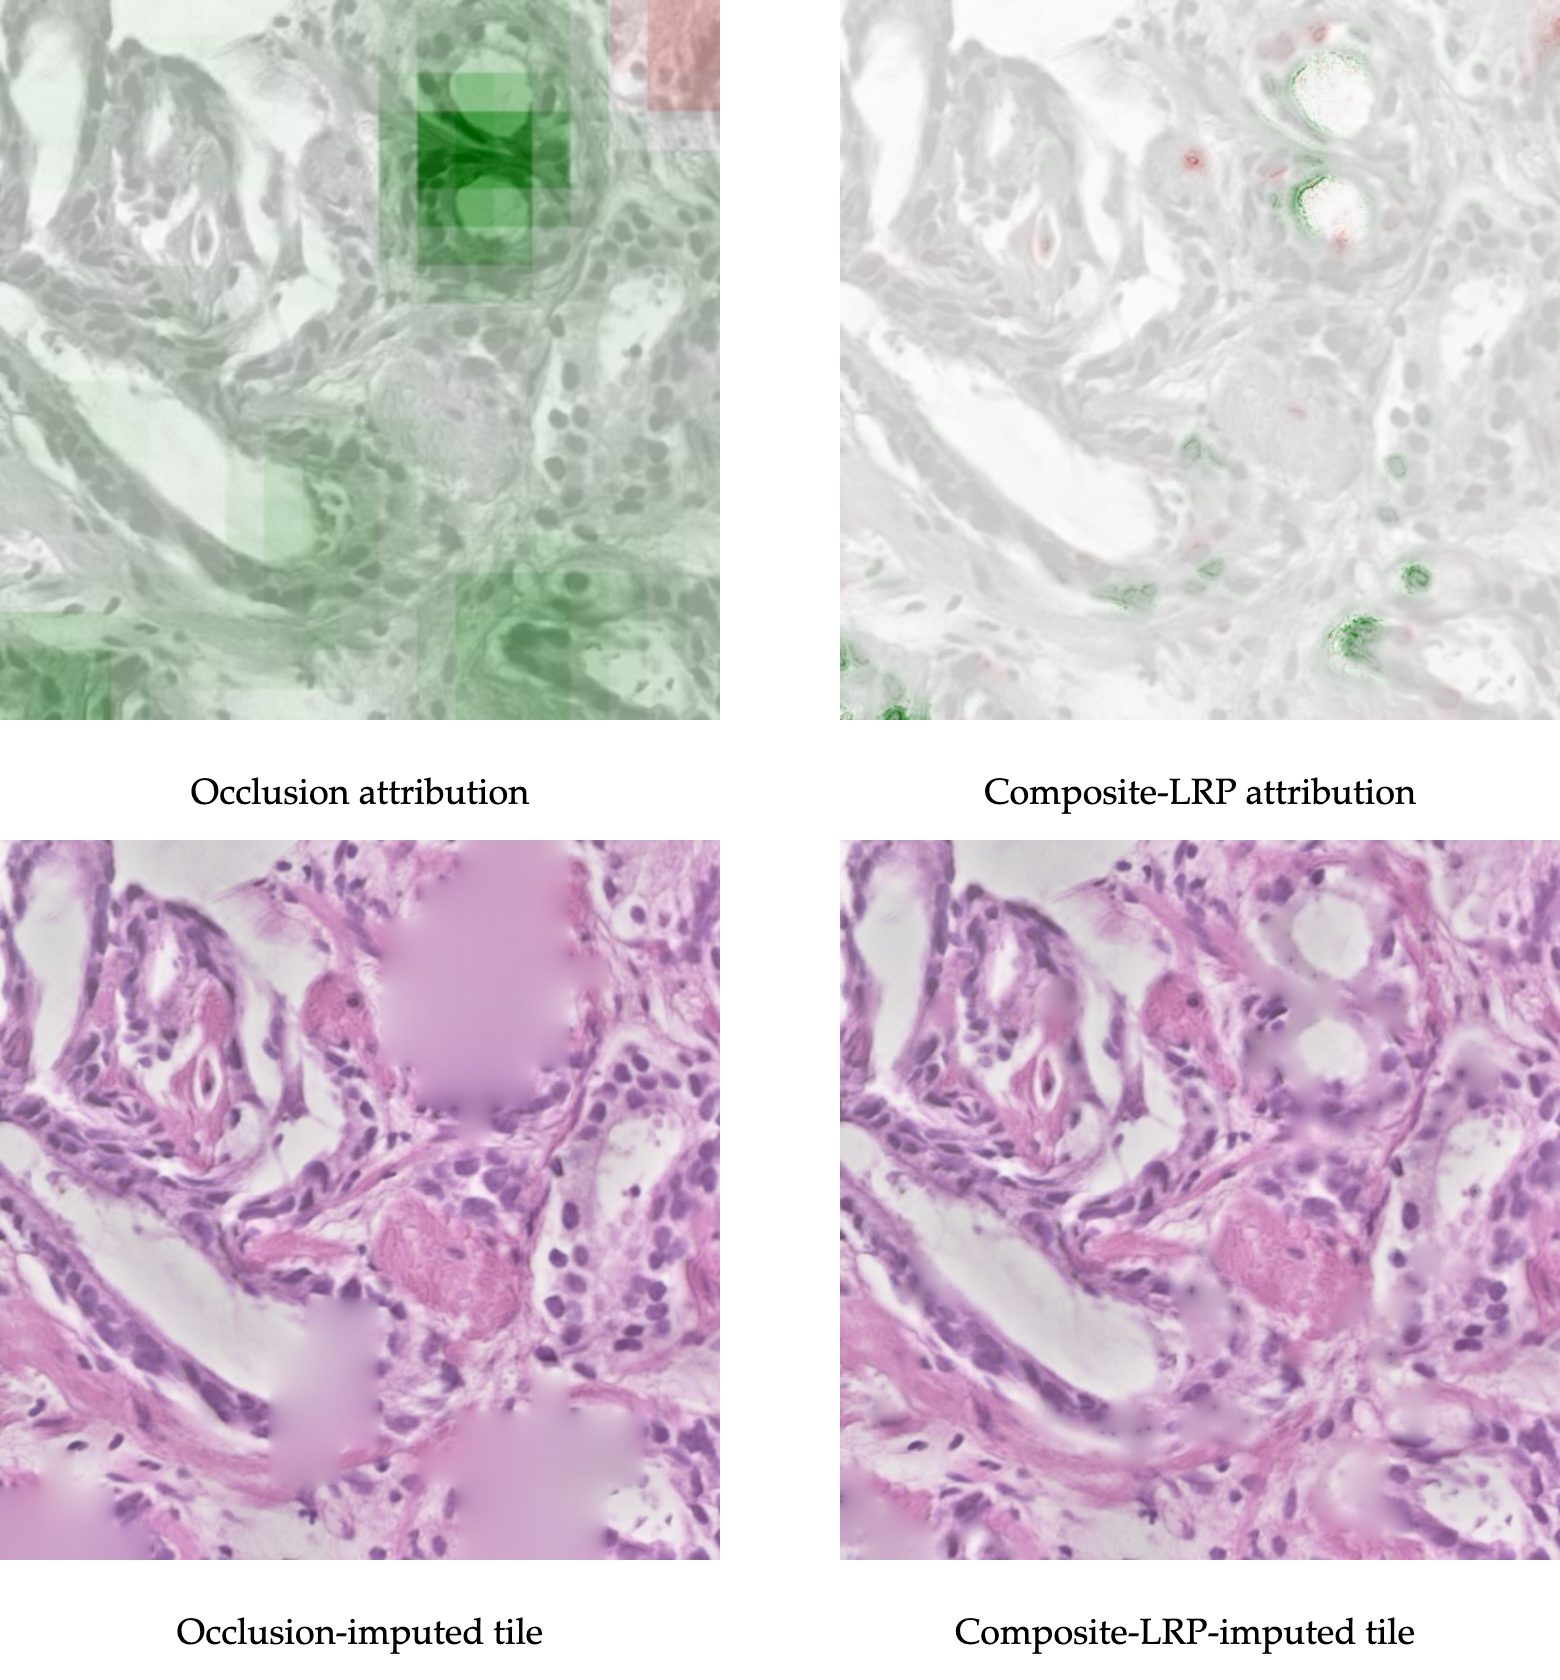
\includegraphics[width=0.8\textwidth]{img/road-impute.png}
    \caption{
    The top row shows the saliency maps for Occlusion and Composite-LRP for the same tile.
    The bottom row shows a visualization of the tile imputed based on the $20$ percent of the most salient attribution pixels.
    While \texttt{NoisyLinearImputer} removes continuous regions based on the Occlusion attribution, the scattered Composite-LRP attribution and subsequent imputation lead to a tile visually very similar to the original one.
    As a result, methods producing less-scattered saliency maps received higher ROAD scores, consistent with results from \cite{gallo}.
    Images featuring attributions are presented in black and white to increase the visual contrast between the tile and the explanation.
    It is important to note that ROAD favors methods that cover larger areas of the tile --- because we are imputing larger regions for the same percentual threshold.
    However, the visualization can be misleading, as in this case, the Composite-LRP positively attributed more than $58$ percent of the tile.
    }
    \label{fig:road-impute}
\end{figure}

\subsection*{Localization}

The faithfulness metric tells us how well the explainability method attributes the most important features for the model's decisions.
In addition, we want to ensure that these features resemble what pathologists would classify as adenocarcinoma.
To measure how well the output of a given method matches the pathologists' annotations, Gallo et al. \cite{gallo} used the Effective Heat Ratio (EHR) \cite{ehr} metric.
EHR relies on ground truth bounding boxes that encapsulate objects of interest.
Because of our specific use case, we argue that EHR is not the most appropriate method.
Given a bounding box, EHR, by design, favors methods that cover larger annotation areas with strong saliency.
Such merits are not necessarily desired, as the bounding box only marks the rough location of cancerous tissue --- precise pixel-level boundaries are challenging to follow \cite{gallo, annotation-agreement}, and such precise annotation would likely vary from pathologist to pathologist \cite{annotation-agreement}.
Therefore, EHR may discriminate methods that point to cancer markers but do not attribute healthy surrounding tissue included in the annotation.

Instead, we will use what we consider to be a simpler technique called Weighting Game \cite{weighting-game}.
It builds upon the established Pointing Game metric \cite{pointing-game}, which looks at whether the most salient pixel falls within a bounding box of the object of interest.
Unlike the Pointing Game, which only gives us binary information about the accuracy of a given method, the Weighting Game calculates the ratio of the mass of the saliency map $S$ within the bounding box to the total mass of the $S$.
Compared to EHR, this does not disqualify methods that highlight smaller parts of the annotated region, and we believe it gives us a fair measure of how the explanation holds up against the pathologist's annotation.
Given a tile $x$, annotation in the form of binary mask depicting the annotated region $A$ and saliency map $S$, the ratio $r$ is calculated as
\begin{equation}\label{eq:wg}
    r = \frac{\operatorname{\text{mass}}(S \odot A)}{\operatorname{\text{mass}}(S)}.
\end{equation}
In \cite{weighting-game}, authors first blur the annotation mask by convolving it with a $3 \times 3$ filter to counter possible imprecision given a pixel-level ground truth bounding boxes.
We decided to omit this blurring step since, given our domain, the annotations are implicitly not ground truth for the exact borders of cancerous tissue, and we already account for such imprecision with the coarser polygon shape of the annotation.

It is essential to understand the role of this metric in our benchmark.
Post-hoc XAI methods act as a proxy between a model and its user.
The model may have errors and hidden biases, so we cannot disregard a method solely on a bad Weighting Game score alone.
Such a method may still reveal important information and help to facilitate such flaws.
However, we believe that our model has an excellent performance, rigorously verified with a domain expert in \cite{gallo}.
We, therefore, see this metric as a bridge between the quantitative faithfulness metric and qualitative but inherently subjective domain expert assessment.

\myref{Figure}{fig:weighting-game-boxplot} shows the ratio distribution per positive tiles in the test part of our dataset.
Since we threshold the Occlusion saliency maps when viewing the WSIs in the browser, we evaluate over different percentages of the most salient pixels retained.
Gradient-based CAMs outperform Occlusion across all thresholds, advocating for the positive influence of gradient on localization capabilities.
CAM performs similarly, slowly catching up as we retain only the most salient attributions.
Composite-LRP starts with a better score than Occlusion, but it improves negligibly as we approach higher percentages of removed saliency, likely meaning that this method focuses on features that do not fall within the annotation mask.


\begin{figure}
    \begin{center}
    \begin{minipage}{1\textwidth}
      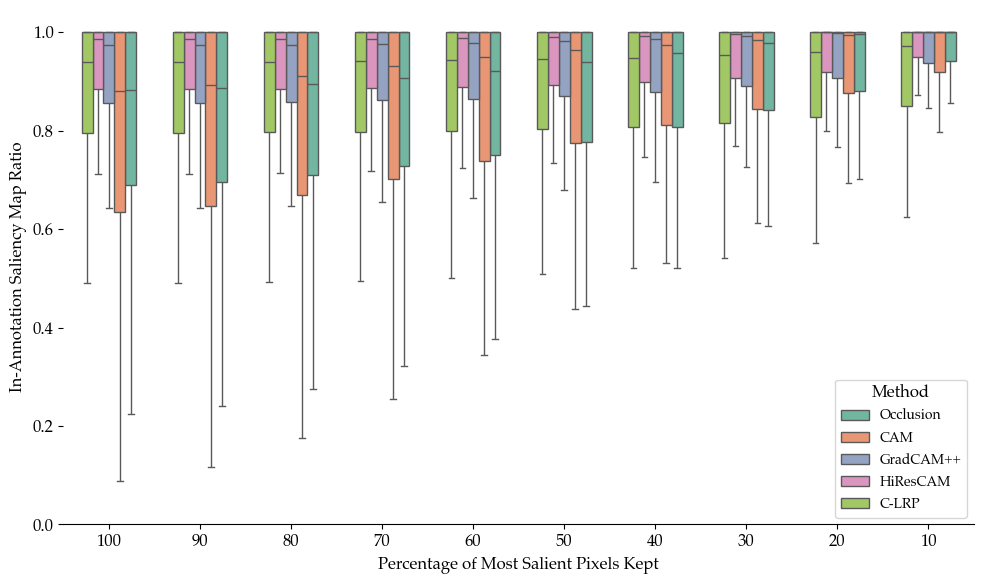
\includegraphics[width=\textwidth]{img/weighting-game-boxplot.png}
    \end{minipage}
    \caption{
    Boxplot of the Weighting Game ratios w.r.t annotations across different percentages of the most salient pixels kept.
    Note the excellent localization capabilities of the gradient-based CAMs right from the start.
    This is not surprising in the case of HiResCAM, as it sums over the strongest activations only, rendering the saliency map more conservative in terms of how much of the tile they cover.
    However, we expected CAM to perform similarly to GradCAM++.
    When we visually inspected where this difference came from, we found that CAM tends to be more liberal with the tile coverage.
    However, the areas where the two methods differ tend to have low saliency, and CAM catches up with GradCAM++ when only the most salient regions are considered.
    The score for Composite-LRP improves very slowly, and this slow improvement likely means that Composite-LRP tends to strongly attribute features that do not fall within the annotated region, and corresponding attributions are preserved even when we keep only the most salient regions.
    }
    \label{fig:weighting-game-boxplot}
    \end{center}
\end{figure}

\subsection*{Usefulness}

The usefulness of an explanation in the context of deep learning models is necessarily subjective, as it varies depending on the individual's perspective and context --- according to \cite{xai-doshi}, the audience's background, expertise, and purpose of use all play critical roles in determining the perceived utility of an explanation --- something hard to capture by a quantitative metric.

Fortunately, we know that Occlusion generates semantically correct saliency maps aligned with features recognized by pathologists \cite{gallo}.
Thus, we will use the Weighting Game metric to assess how well the saliency maps of candidate methods resemble those of Occlusion --- by using binary Occlusion saliency maps as annotations.
During the analysis in a browser, the pathologist adjusts the threshold of the Occlusion slide-level saliency maps to display between approximately $45$ and $25$ percent of the most salient pixels.
However, since Occlusion-based annotations cannot be considered a ground truth for relevant morphological features, we deem this setting too strict for our metric, as some tile-level saliency maps would get completely erased.
This metric assesses whether one of our candidate methods is a suitable proxy similar to Occlusion --- not that it perfectly matches its results, as the pathologist would use them.
Therefore, we will only use tile-level thresholding to make Occlusion saliency maps more conservative regarding how much of a tile they cover.
Experimentally, we chose to keep $45$ percent of the most salient pixels per tile.
Such tile-level thresholding eliminates regions with too-low saliency and still preserves a large portion of the explanation for candidate methods to hit into.
To create an Occlusion-based annotation, we convert the thresholded Occlusion saliency map into a binary mask, where positive values are assigned a value of $1$.
We then use this binary mask map as the annotation $A$ in \myref{Equation}{eq:wg}.

We do not perceive this metric as adding to candidate methods' faithfulness or localization capabilities.
Instead, its purpose is twofold.
First, it guides our selection of which explainability methods to present to a pathologist, allowing us to prioritize explanations that align the most closely with the Occlusion baseline.
Second, it enables us to evaluate how the pathologist subjectively perceives candidate explainability techniques relative to the acceptance of Occlusion.

\myref{Figure}{fig:occ-weighting-game-boxplot} portrays the distribution of Occlusion Weighting Game ratios across different thresholds for candidate saliency maps.
HiResCAM agrees well with Occlusion-based annotation.
The agreement is in line with our a priori expectation from \myref{Subsection}{sub:hirescam} that Occlusion will attribute mainly regions spatially corresponding to the highest activations in activation maps since only those are considered when computing the final score because of GMP.
Although GradCAM++ and CAM produce visually similar results, GradCAM++'s saliency maps tend to hit areas marked by Occlusion better.
However, CAM starts to catch up towards the higher thresholds for disregarded pixels.
Composite-LRP performs consistently across all thresholds, supporting the observation that it assigns saliency to regions not considered important by other methods.

\begin{figure}[t]
    \centering
    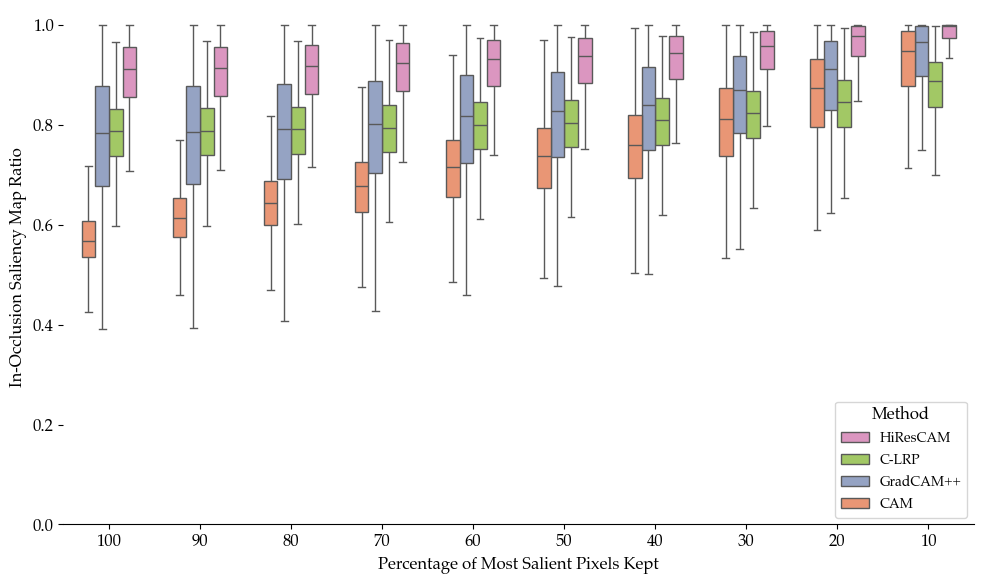
\includegraphics[width=\textwidth]{img/occlusion-weighting-game-boxplot.png}
    \caption{
    Boxplot of the Weighting Game ratios, when we take $45$ percent of the most salient pixels from the Occlusion saliency map as the bounding box.
    Note that HiResCAM achieves high ratios very consistently.
    We attribute the high score to the conservativeness of the areas covered by its saliency maps and our expectation from \myref{Subsection}{sub:hirescam}.
    Despite the similar performance of CAM and GradCAM++ in faithfulness and localization metrics, GradCAM++ tends to better resemble the Occlusion-based annotation until taking only the most salient pixels from respective saliency maps.
    In some cases, Composite-LRP likely focuses on different regions of the image, displaying similar behavior as when we used expert annotations.
    }
    \label{fig:occ-weighting-game-boxplot}
\end{figure}

\section{Domain Expert Assessment}

This section presents a qualitative evaluation of the produced explanations by a domain expert.
In \cite{gallo}, Gallo et al. first generated saliency maps for all test slides.
Then, they sampled a subset of $461$ regions, where Occlusion suggested an area important for the model when deciding whether to be pro or against the presence of cancer.
Initially, we wanted to present candidate saliency maps for all the $461$ original regions.
However, this would implicitly handicap methods, which focus on different, albeit still relevant, parts of the WSI. 
Another option was to create saliency maps of candidate methods for the test set and try to sample new regions of interest.
However, we could not use the original approach as is since it also relied on negative attributions, which we do not have for HiResCAM and GradCAM++.
Furthermore, such sampling could also be unfair, as the distribution of different morphological features would likely vary across different samples.
A rigorous and thorough review of detected cancer markers in hundreds of samples also requires a non-trivial time investment of a domain expert.

With all this in mind, we reviewed the results of our quantitative metrics and decided to reframe the assessment.
We leverage that our domain expert already has prior experience with results based on Occlusion.
Therefore, we generate saliency maps for candidate methods for all test WSIs.
We narrowed down the presented methods based on their quantitative results so as not to waste the pathologist's time.
We decided to include explanations of two methods, CAM and HiResCAM.
CAM has comparable quantitative results to GradCAM++ while being faster.
Unlike GradCAM++, saliency maps from CAM also contain negative regions, pointing to locations the model perceives as against cancer --- same as Occlusion.
Moreover, GradCAM++ gave very different results in \myref{Appendix}{sec:conv-vs-pool}, decreasing our trust in its internal mechanism.
HiResCAM performed particularly well when quantitatively comparing marked salient regions to the Occlusion-based annotations.

In this setting, the target audience is an experienced pathologist, MUDr. Rudolf Nenutil, CSc.
He has a long track record of working with the RationAI group and is one of the authors of \cite{gallo}.
To subjectively assess the usefulness of the saliency maps, we gave him the following task:

\begin{doublebar}
\begin{quote}
In the attached URI, you will find a report with 87 test slides and saliency maps generated by two explainability methods:
\begin{itemize}
    \item Saliency maps of CAM contain green and red regions, with the same meaning as in the case of Occlusion --- green areas denote pro-cancerous features, while red areas denote non-cancerous tissue.
    \item Saliency maps for HiresCAM are in yellow, depicting only the pro-cancerous areas.
\end{itemize}
Please determine whether CAM or HiresCAM saliency maps are a viable replacement for Occlusion:
\begin{enumerate}
    \item Open them in the WSI browser and subjectively assess whether they could be used instead of the Occlusion saliency maps.
    \item As for Occlusion, find a suitable threshold such that the saliency points to the relevant morphological features.
    \item Assess whether those methods point to features and patterns you understand.
    \item Document your findings, noting where the saliency maps align well or poorly with your understanding of the tissue morphology.
\end{enumerate}
We do not expect you to go through all slides --- please do it to the extent that allows you to draw a confident conclusion about the suitability of candidate methods.
\end{quote}
\end{doublebar}
We deliberately did not display the Occlusion maps to avoid biasing MUDr. Nenutil.
This section aims to assess how well the candidate maps represent known morphological patterns --- we have already compared the Occlusion similarity quantitatively.

MUDr. Nenutil gave us a presentation, which is included in supplementary materials.
In this presentation, he annotated several regions of interest for our model proxied by CAM and HiResCAM.
He used the concept of \emph{xPatterns} --- ``seven prominent patterns, four
typically forming pro-cancer morphological features and three typical
for non-cancer tissue'' --- from~\cite{gallo}.

CAM detects $4/4$ pro-cancer and $3/3$ non-cancer xPatterns.
HiResCAM, comprised only of positive saliency, can detect $4/4$ pro-cancer xPatterns identified in \cite{gallo}.
Both methods detect the same pro-cancer patterns, consistent with their theoretical background presented in \myref{Section}{sec:xai-cnn}.
\myref{Figure}{fig:both-pos} and \myref{Figure}{fig:both-nuclear-density} show positive patterns detected by CAM and HiResCAM.
Negative xPatterns detected by CAM are shown in \myref{Figure}{fig:cam-neg}.
All saliency maps in presented images are thresholded so that we display only the $70$ percent of the most salient pixels.

According to the subjective evaluation by MUDr. Nenutil, ``CAM is more sensitive to `High nuclear density' positive pattern'' while ``HiresCAM is more sensitive to `Single chain of nuclei' and `Larger nucleus with perinuclear halo' patterns, which results in much more false positive labels''.
This observation is illustrated in \myref{Figure}{fig:both-pos}, and we posit it positively advocates for the trustworthiness of our model. 
Those two methods help to show that while the model correctly perceives most features as negative, it can still detect and recognize a feature advocating for cancer.
However, given other contextual information, it is disregarded, and the model correctly classifies the tile as non-cancerous, as shown in \myref{Figure}{fig:ruda-annot}.

\begin{figure}
    \centering
    \includegraphics[width=1\textwidth]{img/all-methods.png}
    \caption{
    Comparison of thresholded and raw Occlusion saliency maps with annotated CAM and HiResCAM.
    In line with our expectations, HiResCAM focuses on the same regions as thresholded Occlusion and detects more instances of the same pattern.
    CAM assigns a negative saliency in places where Occlusion reports slightly positive regions, but these slightly positive regions are removed during thresholding.
    Moreover, after a discussion with MUDr. Nenutil, we discovered that the negative regions reported by CAM correspond to the negative ``Areas of low nuclear density with eosinophilic background'' xPattern, meaning that, unlike Occlusion, CAM correctly reports negative saliency.
    Both candidate methods successfully detect and report all positive xPatterns from \cite{gallo}, even though there are only $3$ present in this image.
    Note that in areas where CAM reports negative attributions due to a prevalence of healthy tissue, HiResCAM still correctly points out relevant pro-cancer morphological features, namely larger nuclei with perinuclear halos.
    Annotated images taken from the presentation of MUDr. Nenutil, which is available in the supplementary material.
    }
    \label{fig:both-pos}
\end{figure}

\begin{figure}
    \begin{center}
    \begin{minipage}{1\textwidth}
    %\fcolorbox{RoyalBlue}{white}
      {\includegraphics[width=0.49\textwidth]{img/cam-nuclear-density.png}
      \includegraphics[width=0.49\textwidth]{img/hirescam-nuclear-density.png}}
    \end{minipage}
    \caption{
    Coverage of the ``High nuclear density'' xPattern from \cite{gallo}.
    MUDr. Nenutil assessed that CAM, on the left, is more sensitive to this particular xPattern.
    This is due to HiResCAM's internal mechanism of preserving only the strongest activation per activation map.
    Therefore, although the activation maps for corresponding xPattern are largely filled with positive values, most are not reflected in the resulting saliency map, and the map looks diluted and scattered.
    }
    \label{fig:both-nuclear-density}
    \end{center}
\end{figure}

\begin{figure}
    \begin{center}
    \begin{minipage}{0.8\textwidth}
    %\fcolorbox{RoyalBlue}{white}
      {\includegraphics[width=\textwidth]{img/cam-neg.png}}
    \end{minipage}
    \caption{
    CAM can correctly detect the presence of $3/3$ negative xPatterns from \cite{gallo}.
    The identification of negative attributions is often overlooked by other CAM-based methods.
    We believe this is due to the fact that, given a classifier trained to distinguish between hundreds of classes, information about what in the given image advocates \emph{against} the class of interest may be very difficult to interpret.
    In our binary classifier setting, a proxy showing negative attribution can provide a comprehensible result consistent with the concepts relevant to a domain expert.
    }
    \label{fig:cam-neg}
    \end{center}
\end{figure}

\begin{figure}
    \centering
    %\fcolorbox{RoyalBlue}{white}
      {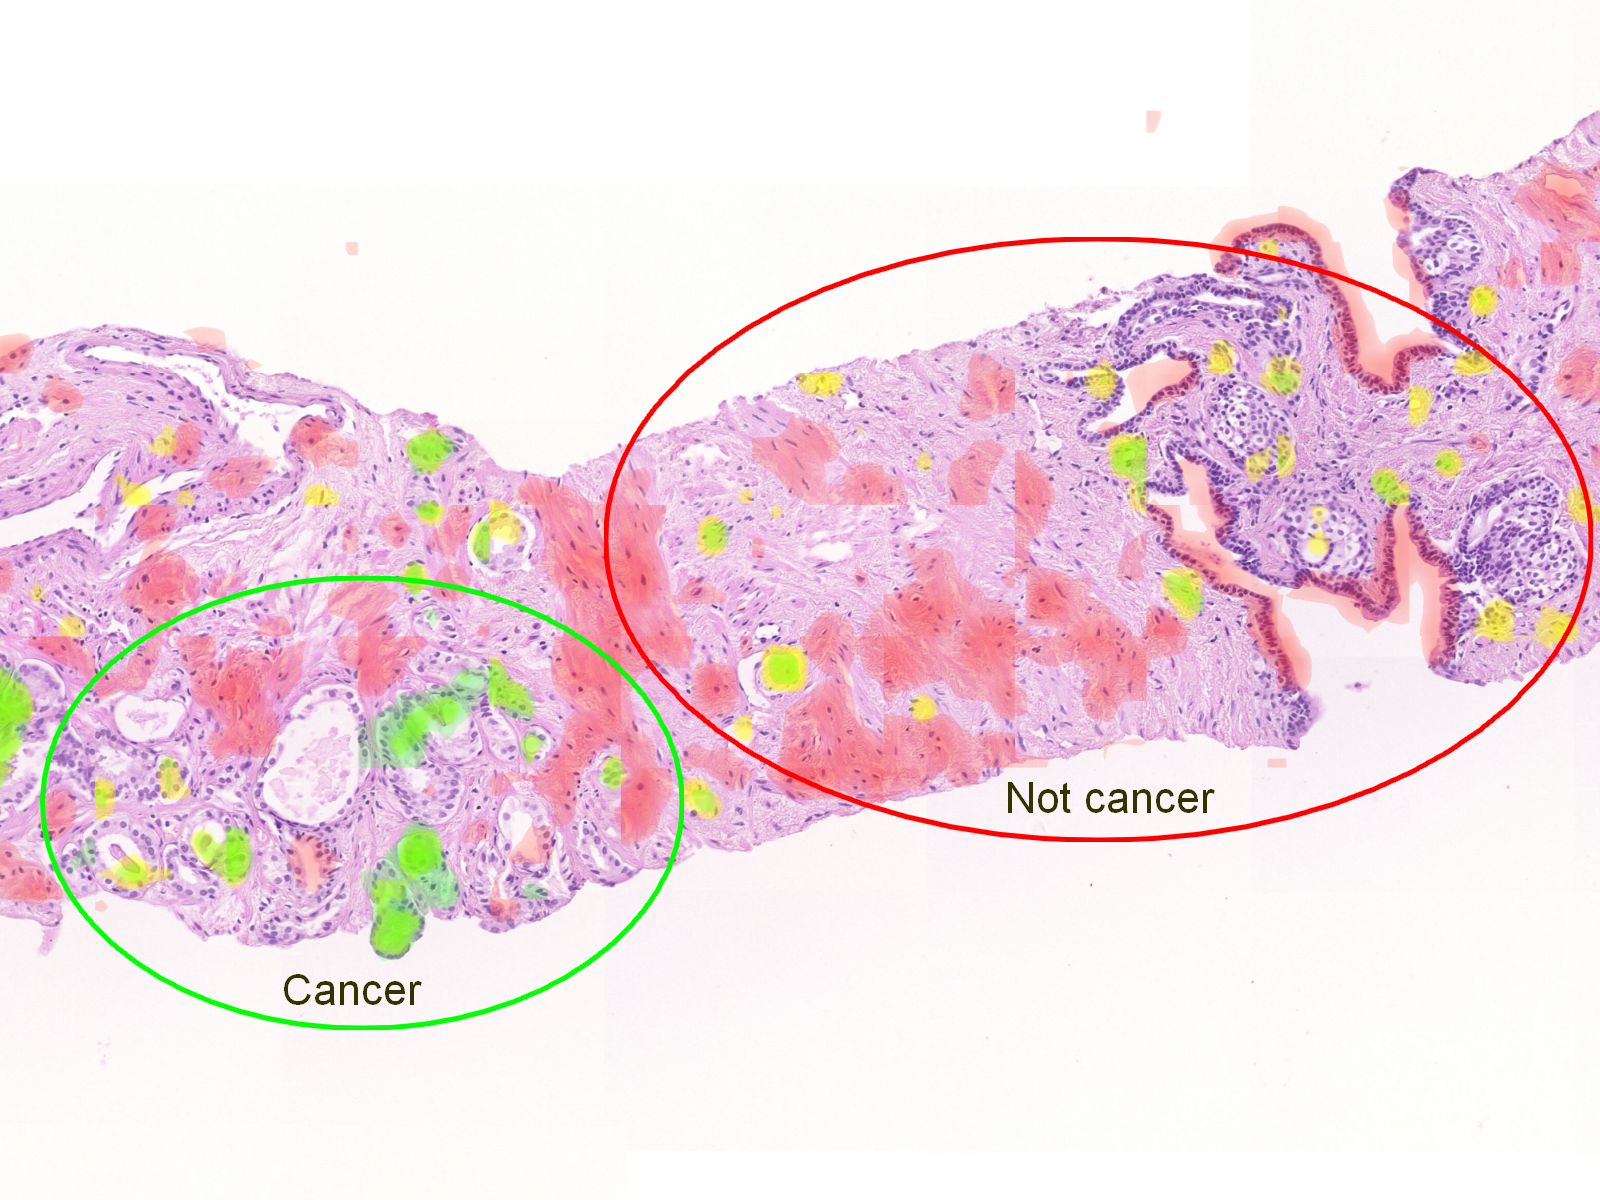
\includegraphics[width=\textwidth]{img/ruda-annot.png}}
    \caption{
    Image with annotation by MUDr. Nenutil, showing cancerous and non-cancerous areas.
    Both CAM and HiResCAM assign positive saliency to the cancerous area, with both methods highlighting the same features.
    In the non-cancerous part, CAM indicates the prevalence of features considered against the presence of cancer by our model.
    HiResCAM, taking only the strongest activations per unit into account, still displays relevant positive regions of interest in the non-cancerous region.
    We posit that combining these methods can help us debug the model and quickly distinguish between situations where the model has failed to detect a pattern and where the pattern has been detected, but the model disregards it because of surrounding healthy tissue.
    }
    \label{fig:ruda-annot}
\end{figure}